\documentclass{article}

% If you're new to LaTeX, here's some short tutorials:
% https://www.overleaf.com/learn/latex/Learn_LaTeX_in_30_minutes
% https://en.wikibooks.org/wiki/LaTeX/Basics

\def\rd{{\rm d}}
\def\ds{\displaystyle}

% Formatting
\usepackage[utf8]{inputenc}
\usepackage[margin=1in]{geometry}
\usepackage[titletoc,title]{appendix}

% Math
% https://www.overleaf.com/learn/latex/Mathematical_expressions
% https://en.wikibooks.org/wiki/LaTeX/Mathematics
\usepackage{amsmath,amsfonts,amssymb,mathtools}

% Images
% https://www.overleaf.com/learn/latex/Inserting_Images
% https://en.wikibooks.org/wiki/LaTeX/Floats,_Figures_and_Captions
\usepackage{graphicx,float}

% Tables
% https://www.overleaf.com/learn/latex/Tables
% https://en.wikibooks.org/wiki/LaTeX/Tables

% Algorithms
% https://www.overleaf.com/learn/latex/algorithms
% https://en.wikibooks.org/wiki/LaTeX/Algorithms
\usepackage[ruled,vlined]{algorithm2e}
\usepackage{algorithmic}

% Code syntax highlighting
% https://www.overleaf.com/learn/latex/Code_Highlighting_with_minted
\usepackage{minted}
\usemintedstyle{borland}

% References
% https://www.overleaf.com/learn/latex/Bibliography_management_in_LaTeX
% https://en.wikibooks.org/wiki/LaTeX/Bibliography_Management
\usepackage{biblatex}
\addbibresource{references.bib}

% Title content
\title{AMATH 482 Homework 3}
\author{Yiping Li}
\date{February 24, 2021}

\begin{document}

\maketitle

% Abstract
\begin{abstract}
    The goal of this study is to illustrate the various aspects of the Principle Component Analysis (PCA). We are given. In the study, we are given several recordings of a spring-mass system from various angle under different conditions, and we are asked to use the PCA to extract the dynamics of the system. The traits and usefulness of the PCA will be evaluated and compared based on the extractions.
\end{abstract}

% Introduction and Overview
\section{Introduction and Overview}
% Example Subsection
\subsection{Problem Setting}
The spring-mass system is recorded under four conditions: ideal case, noisy case, horizontal displacement, and horizontal displacement with rotation. For each case, there are three camera recording the system from difference angle. \\
~\\
Since we want to analyze the dynamics of the system, we have to extract the positions of the object from the videos, and it is also one of the big obstacles we faced. \\
~\\
As previously mentioned, our task is to break down the dynamics of the system. The PCA will allow us to separate different independent motions, for examples, vertical single harmonic motion done by the mass and rotation of the mass.
% Example Subsubsection
\subsection{Data Format}
All the recordings has the resolution of 480*640, which means that for each frame (image), there are 480 rows, and each row has 640 pixels. The recordings are loaded as \texttt{4-D unit8} objects in \textbf{MATLAB}. All recordings has different length, which means that some videos have more frames than other ones.
~\\
In the video, a spring-mass system was displayed. A paint bucket was hanging under a spring. A flashlight was tuned on and placed on the paint bucket. Besides, the first two cameras were placed normally, but the third camera was turned sideways.
%  Theoretical Background
\section{Theoretical Background}
The mathematical side of the PCA is supported by the Singular Value Decomposition (SVD). SVD demonstrates that for any given matrix \textbf{A}, we can decomposition it as,
\[
\mathbf{A} = \mathbf{U\Sigma V^*}
\]
Where $\mathbf{\Sigma}$ is a diagonal matrix, and $\mathbf{U}$ and $\mathbf{V}$ are both orthogonal matrices. Those three matrices can be calculated from two eigenvalue problem.
\begin{equation}
    \begin{aligned}
    \mathbf{AA^{*}} &=\mathbf{U\Sigma V^*}\mathbf{U\Sigma V^*}^*\\
    \mathbf{AA^{*}} &=\mathbf{U\Sigma V^*V\Sigma U^*} \\
    \mathbf{AA^{*}} &=\mathbf{U\Sigma^2 U^*} \\
    \mathbf{AA^{*}U} &=\mathbf{U\Sigma^2} \\
    \end{aligned}
\end{equation}

\begin{equation}
    \begin{aligned}
    \mathbf{A^{*}A} &=\mathbf{U\Sigma V^*}^*\mathbf{U\Sigma V^*}\\
    \mathbf{A^{*}A} &=\mathbf{V\Sigma U^*}\mathbf{U\Sigma V^*}\\
    \mathbf{A^{*}A} &=\mathbf{V\Sigma^2  V^*}\\
    \mathbf{A^{*}AV} &=\mathbf{V\Sigma^2}\\
    \end{aligned}
\end{equation}
$\mathbf{\Sigma^2}$ is the eigenvalues of $\mathbf{AA^{*}}$, and the colums of $\mathbf{U}$ and $\mathbf{V}$ are the eigenvectors of matrices $\mathbf{AA^{*}}$ and $\mathbf{A^{*}A}$ respectively. \\
~\\
Similar to the eigen decomposition, the SVD here is also changing the basis, but the SVD Guarantee that the basis is orthogonal, which is the most important feature. The PCA is basically the same as the SVD but in different aspects. \\
~\\
In statistics, we used a parameter called variance to estimate the variability within the samples, which is defined as
\[
\sigma^2 = \frac{1}{\sqrt{n-1}}\sum (x-\mu_x)^2.
\]
Here, $x$ is a random variable and $\mu_x$ is the sample mean of $x$. Therefore, if we subtract the mean before hand and write the data in the sample as a vector $X$, we can rewrite it as,
\[
\sigma^2 = \frac{1}{\sqrt{n-1}}XX^T.
\]
Now, suppose we have two random variables $x_1$ and $x_2$, therefore we can write their samples as $X_1$ and $X_2$. If we want to measure how variables vary with respect to each other, we can calculate there co-variance, which is defined as following,
\[
\sigma_{12}^2 = \frac{1}{\sqrt{n-1}}X_1X_2^T.
\]
If we have several random variables $x_1$ to $x_2$, we can represent them as a matrix $\mathbf{X}$, where $\mathbf{X}=[X_1, X_2, \dots, X_n]^T$. The variance and the covariance of the data can be given by,
\[
\sigma_X^2 = \frac{1}{\sqrt{n-1}}\mathbf{X}\mathbf{X}^T.
\]
Next, suppose we define a matrix $\mathbf{A}=1/\sqrt{n-1}\mathbf{X}$ and apply the SVD, we can get
\[
\mathbf{A} = \mathbf{U\Sigma V^*}
\]
Notice that, the matrix $\mathbf{U}$ allow us transform the data into the new basis, therefore let $\mathbf{Y}$ to be the transformed data, which  $\mathbf{Y} = \mathbf{U^T*X}$. The variances and covariances of $\mathbf{Y}$ is defined as
\begin{equation}
    \begin{aligned}
        \sigma_Y^2 &= \frac{1}{\sqrt{n-1}}\mathbf{Y}\mathbf{Y}^T \\
        \sigma_Y^2 &= \frac{1}{\sqrt{n-1}}\mathbf{U^TX}\mathbf{U^TX}^T \\
        \sigma_Y^2 &= \frac{1}{\sqrt{n-1}}\mathbf{U^TXX^TU} \\
        \sigma_Y^2 &= \mathbf{U^T}\frac{1}{\sqrt{n-1}}\mathbf{XX^TU} \\
        \sigma_Y^2 &= \mathbf{U^TAA^TU} \\
        \sigma_Y^2 &= \mathbf{U^T(U\Sigma V^T) (V\Sigma U^T)U} \\
        \sigma_Y^2 &= \mathbf{(U^TU)\Sigma (V^TV)\Sigma (U^TU)} \\
        \sigma_Y^2 &= \mathbf{\Sigma^2} \\
    \end{aligned}
\end{equation}
The computation above shows that the variances of this transformed data $\mathbf{Y}$ is given by the $\mathbf{\Sigma}$ we computed from applying the SVD on $\mathbf{A}$. As previously mentioned, the $\mathbf{\Sigma}$ is a diagonal matrix, which indicate that the $\mathbf{\sigma_Y^2}$ is all zeros expect for the values on the diagonal line. In other words, the covariance of the transformed data $\mathbf{Y}$ is all zero! The variability of one random variable does NOT depend on any other random variables. Therefore, this transformed data $\mathbf{Y}$ will gives us independent or uncorrelated variables in statistics and a orthogonal basis in mathematics. \\
~\\
Thus, the PCA allows us to break down a data set, to see what components does the data set consist of (what are the components that explain the variation in the data set.
% Algorithm Implementation and Development
\section{Algorithm Implementation and Development}
\subsection{Preparation}
By watching the video, we notice that there is a flashlight placed on the mass, therefore we can use this white point generated by the flashlight as the indicator of the position of the mass. However, the recordings also captured a white wall. To reduce the error, we decided to trim the frame so that we can only focus on the white pixels in certain area. We spent lots of time determining a suitable filter by watching them repeatedly. \\
~\\
In this section, we load the videos and initialized the filters for each of the camera.
\begin{algorithm}
\begin{algorithmic}
    \STATE{Loading the videos from \texttt{camXY.mat}}
    \STATE{Define the three filters for trimming the video frame}
\end{algorithmic}
\caption{Preparation}
\end{algorithm}


\subsection{Extracting the position of the mass from the videos}
In this section, we firstly turned each frame into a gray-scale image, which givens a 480 * 640 matrix where elements are integers between 0-255. The higher the value is, the whiter the pixel will be. \\
~\\
Originally, we tried to use \texttt{max} to capture the position, but the plot it generated is not smooth enough since the maximum pixel is not necessarily the center of the light. As for the results, we took out of the pixels that are above a threshold, and record the mean of their coordinate as the position of the mass. \\
~\\
Moreover, the videos all have different length, if we want to put them into one matrix, we have to cut them to make sure they all have the same size.\\
\begin{figure}[h]
    \centerline{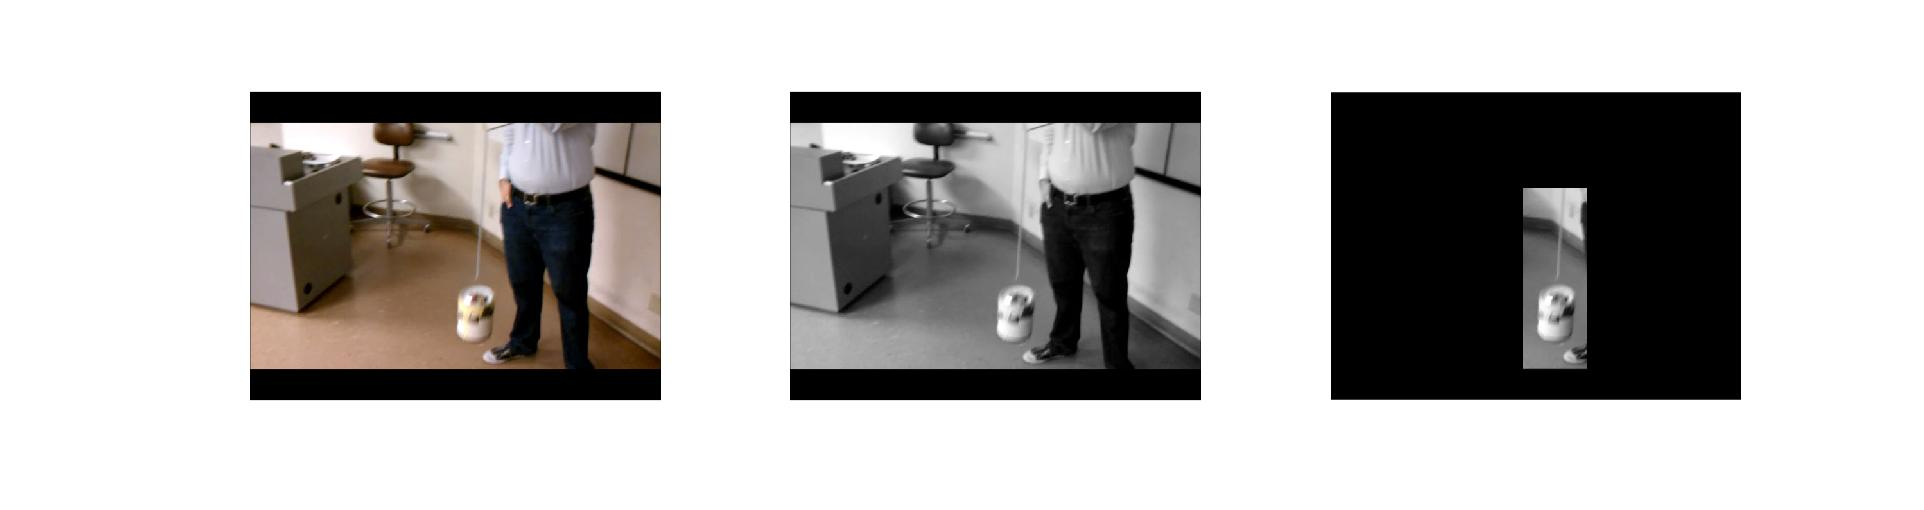
\includegraphics[width=6in]{filter.jpg}}
    \caption{original frame (left), gray-scaled frame (middle), filter we applied (right)}
\end{figure}\\

\begin{algorithm}
\begin{algorithmic}
    \STATE{Define the video set}
    \STATE{Define the filter set}
    \STATE{Define the threshold set}
    \STATE{Find the minimum frame count out of the three videos}
    \FOR{i = 1 to 3}
        \STATE{Define the video}
        \STATE{Define the filter}
        \FOR{i = 1 to minimum frame}
            \STATE{Extract the image at that frame}
            \STATE{Turn it into gray-scale}
            \STATE{Apply the filter}
            \STATE{Find the indices of pixels where the value is greater than threshold}
            \STATE{Record the mean of those indices}
        \ENDFOR
    \ENDFOR
    \STATE{Construct the matrix contains the data}
\end{algorithmic}
\caption{Extracting the position of the mass from the videos}
\end{algorithm}


\subsection{Modifying the data}
Since all videos have different length, they probably are recorded at different time interval. To make sure they are describing the same moment, we tried to trim some frames so that the sine wave they generated are in phase.
\begin{algorithm}
\begin{algorithmic}
    \FOR{i = 1 to 3}
        \STATE{Find the frame where the pixel has the maximum Y-coordinate in first 50 frames}
        \STATE{Keep the 150 frames after that frame}
    \ENDFOR
\end{algorithmic}
\caption{Modifying the data}
\end{algorithm}

\subsection{Apply the SVD}
Now, we had everything set up, we just to break down the data by applying the SVD.
\begin{algorithm}
\begin{algorithmic}
    \STATE{For each row, subtract the mean of that row.}
    \STATE{Divide the matrix by $\sqrt{n-1}$}
    \STATE{Apply the SVD by \texttt{svd}}
    \STATE{Calculate the rank-1 and rank-2 approximation}
    \STATE{Plotting}
\end{algorithmic}
\caption{Apply the SVD}
\end{algorithm}


\section{Computational Result}
\subsection{Test 1: Ideal case}
\begin{figure}[h]
    \centerline{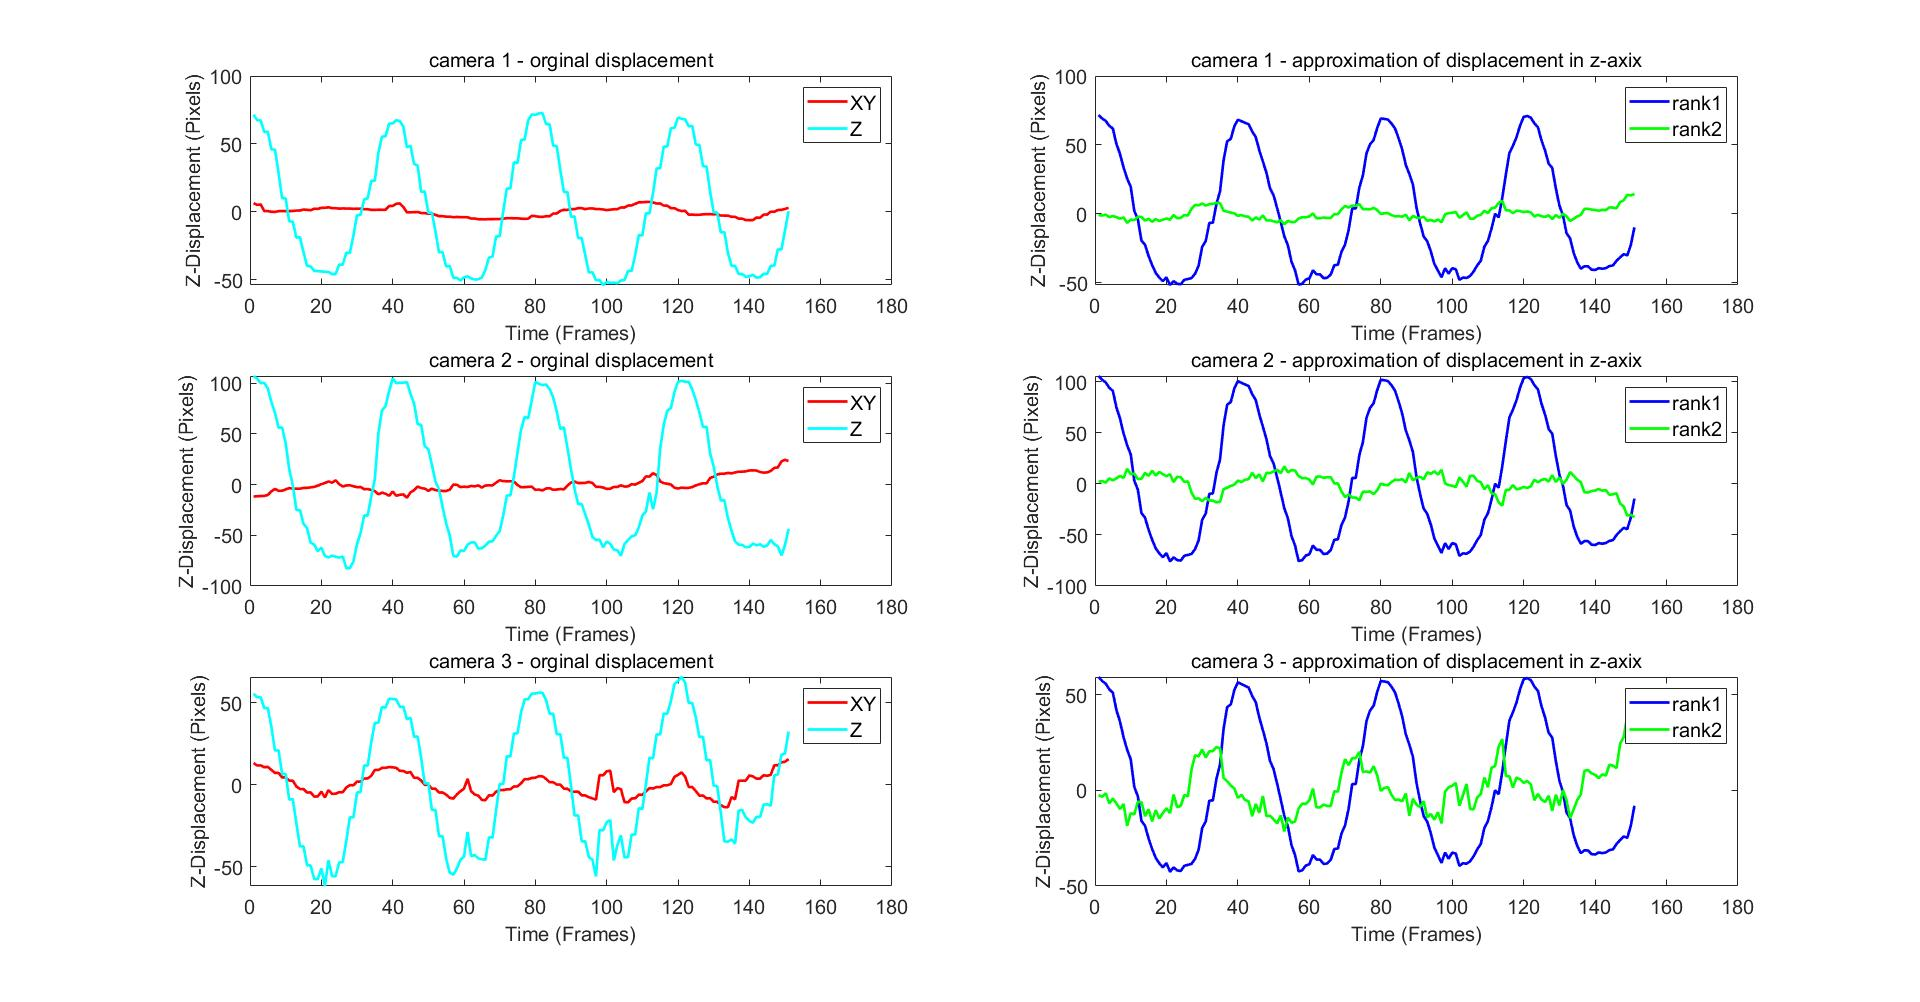
\includegraphics[width=8in]{case11.jpg}}
    \caption{The original displacement and its principle components}
    \centerline{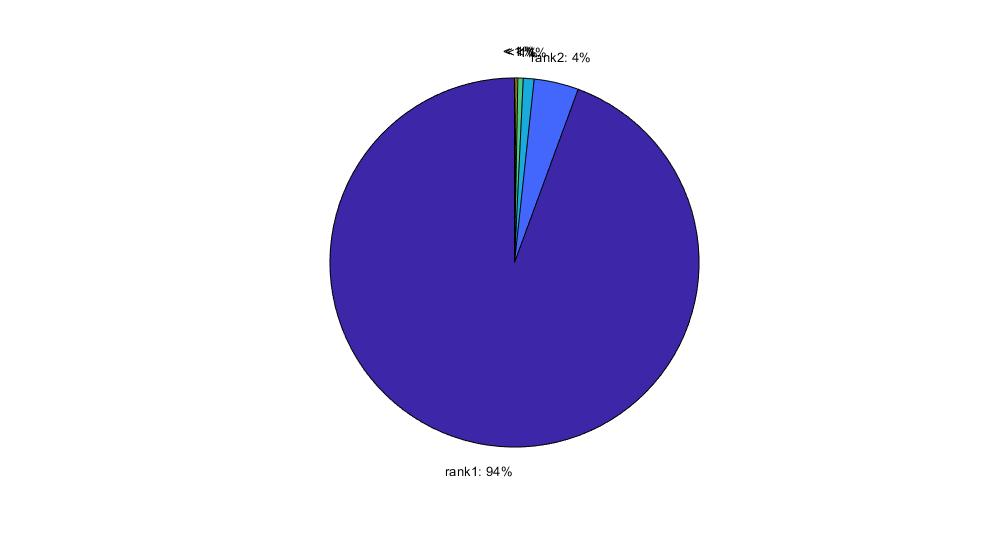
\includegraphics[width=3in]{case12.jpg}}
    \caption{The components of variance in the data}
\end{figure}
\begin{figure}[h]
    \centerline{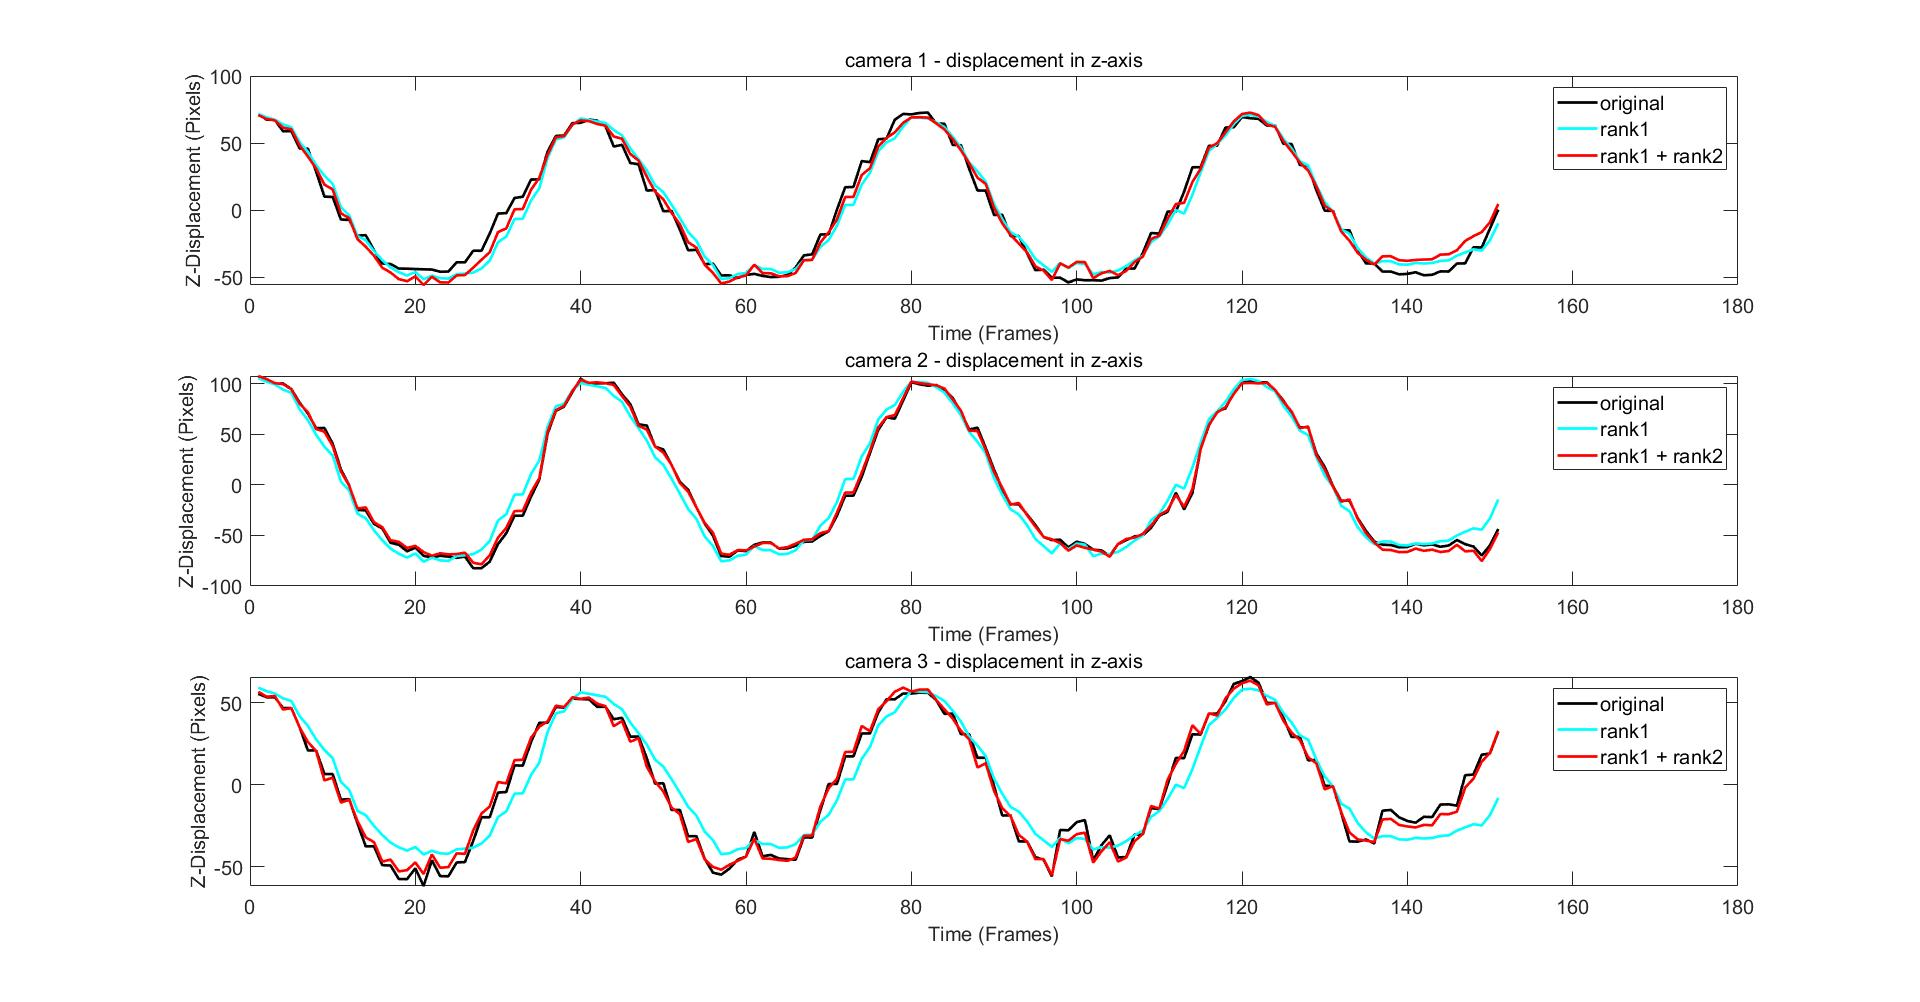
\includegraphics[width=8in]{case13.jpg}}
    \caption{Comparison on the z-direction displacement between real and approximation}
\end{figure}
From Figure 2, we can see that the original plot of the displacement in \textbf{Z} gives us a well-formed sine curve, and the  displacement in \textbf{XY} is almost a horizontal line at $y=0$. As for the third camera, there are some perturbations since it was recording at a bad angle.\\
~\\
From Figure 3, we can see that the first component contribute the most part of the variance ($94\%$). We can also come up with the similar conclusion from Figure 2 and Figure 4.\\
~\\
From Figure 4, we can see that the rank-1 approximation (first components) is already a pretty good fit of the original curve, which is also what we expected since there is only one motion in this ideal case.\\

\subsection{Test 2: Noisy case}
\begin{figure}[h]
    \centerline{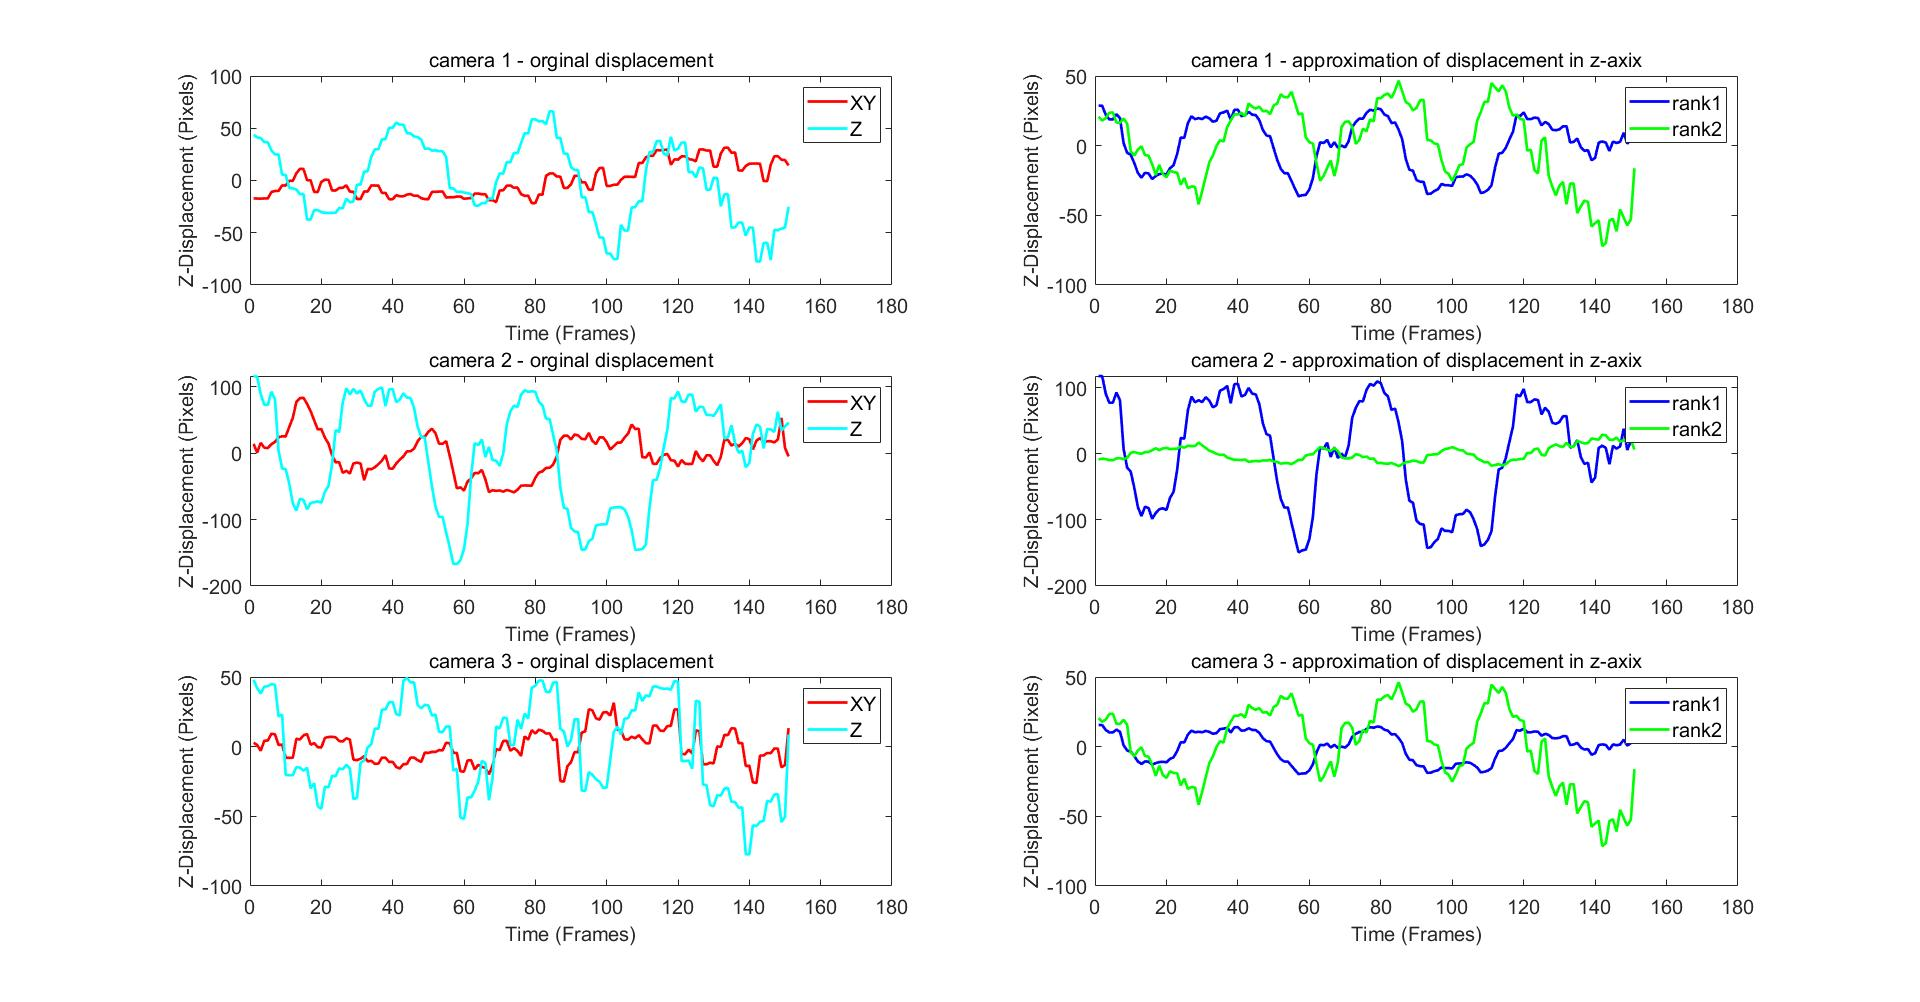
\includegraphics[width=8in]{case21.jpg}}
    \caption{Test 2: Noisy Case - The original displacement and its principle components}
    \centerline{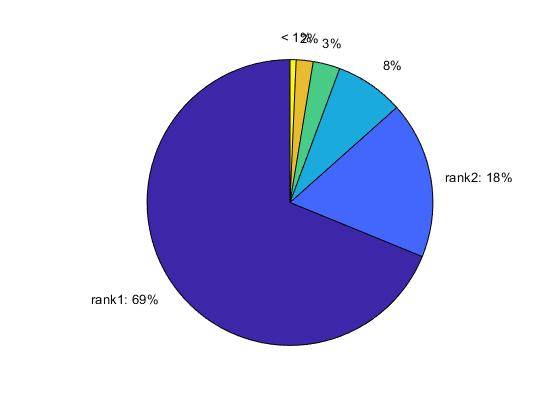
\includegraphics[width=3in]{case22.jpg}}
    \caption{Test 2: Noisy Case - The components of variance in the data}
\end{figure}
\begin{figure}[h]
    \centerline{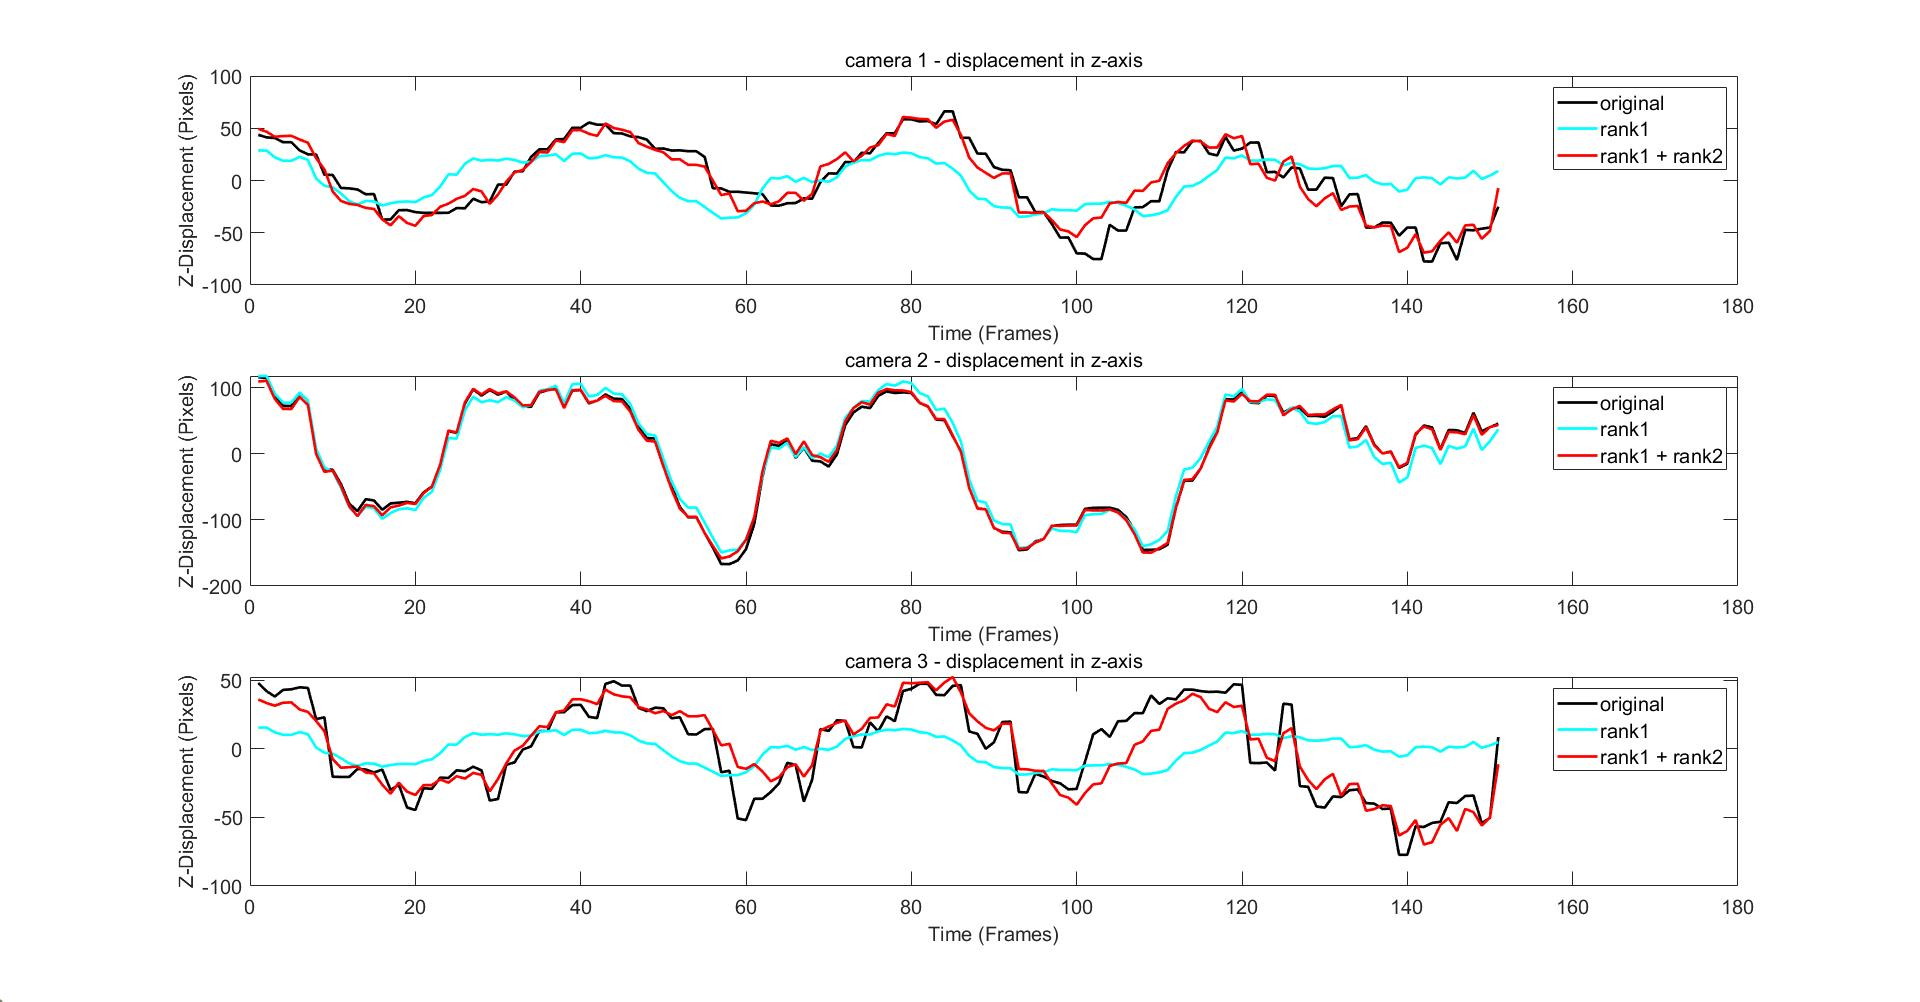
\includegraphics[width=8in]{case23.jpg}}
    \caption{Test 2: Noisy Case - Comparison on the z-direction displacement between real and approximation}
\end{figure}
We still are able to see that the curve is sort on in sine from, but it is much more chaotic than the test 1. Moreover, The decomposition is not like the first case where first component is doing everything. The first component contribute $69\%$ of the variance and the second component contribute $18\%$ of it.
~\\
From Figure 7, we notice that the rank-1 approximation is good on camera 2. As for camera 1 and 3, the rank-2 approximation has to be added to construct a good approximation.

\subsection{Test 3: Horizontal Displacement}
\begin{figure}[h]
    \centerline{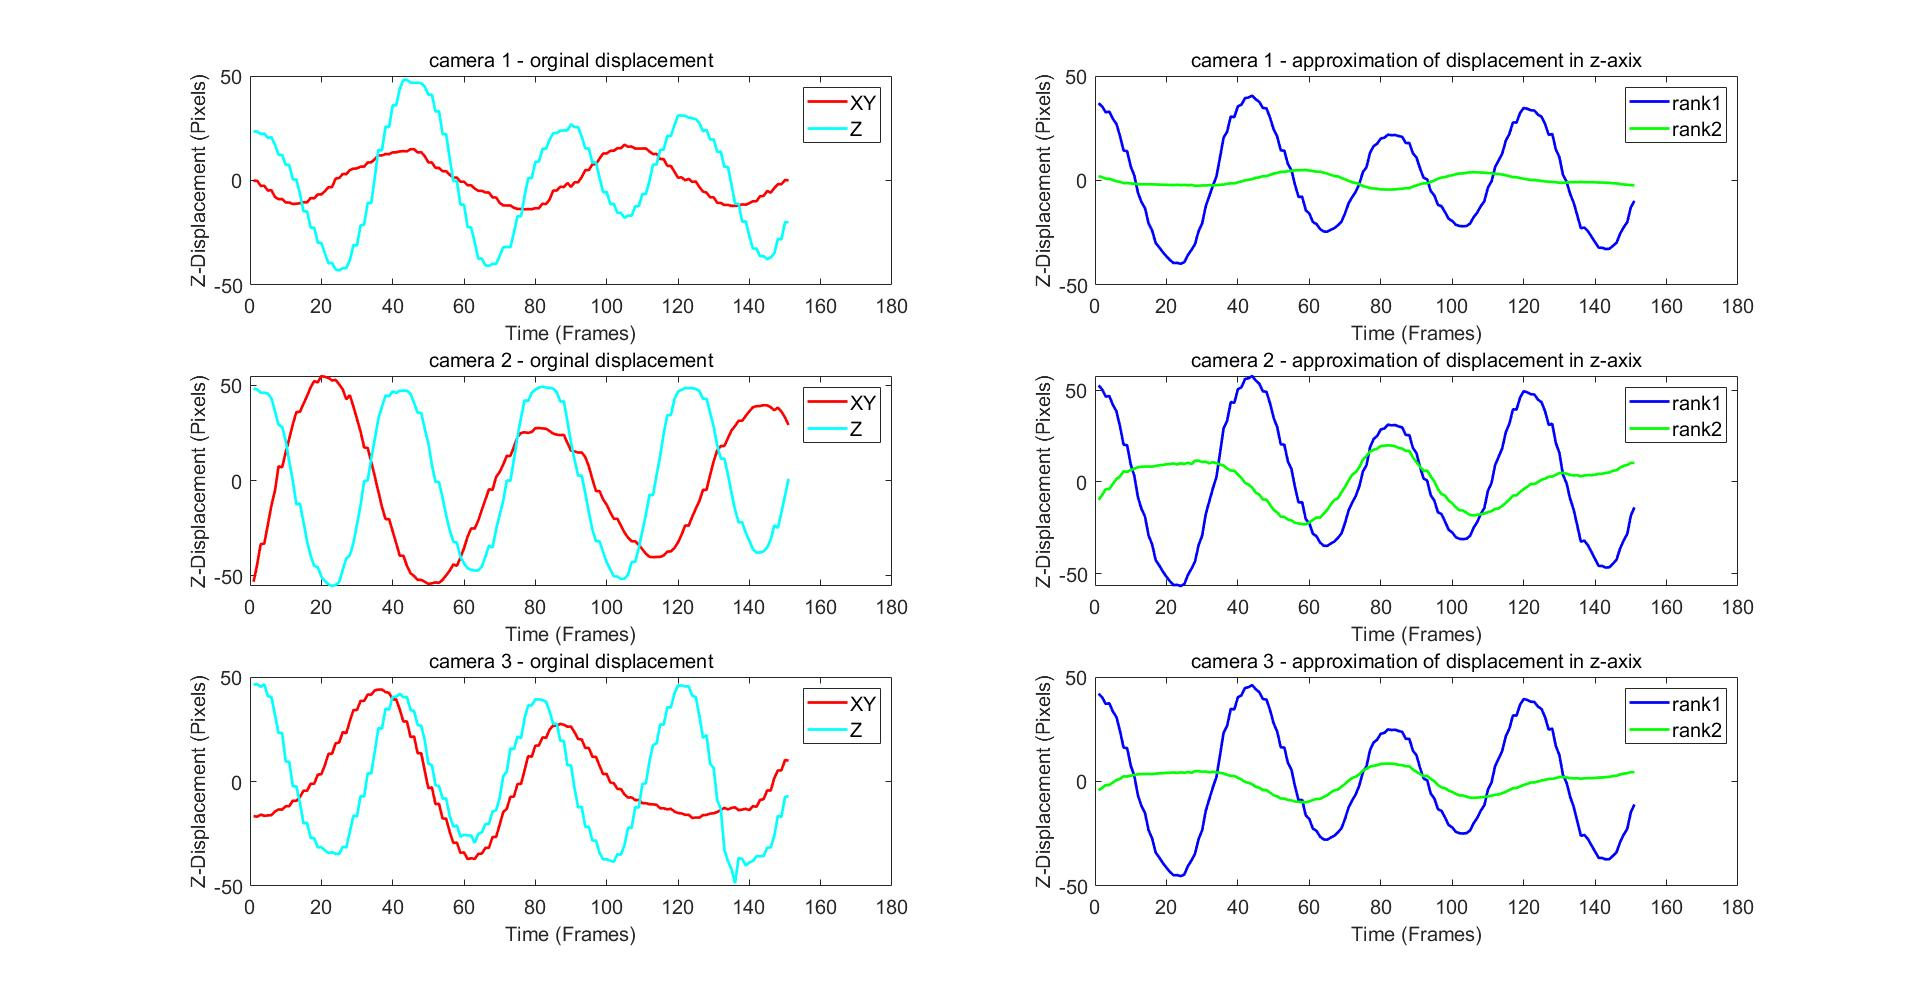
\includegraphics[width=8in]{case31.jpg}}
    \caption{Test 3: Horizontal Displacement - The original displacement and its principle components}
    \centerline{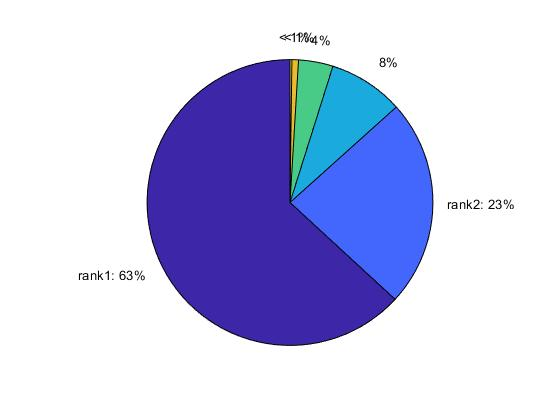
\includegraphics[width=3in]{case32.jpg}}
    \caption{Test 3: Horizontal Displacement - The components of variance in the data}
\end{figure}
\begin{figure}[h]
    \centerline{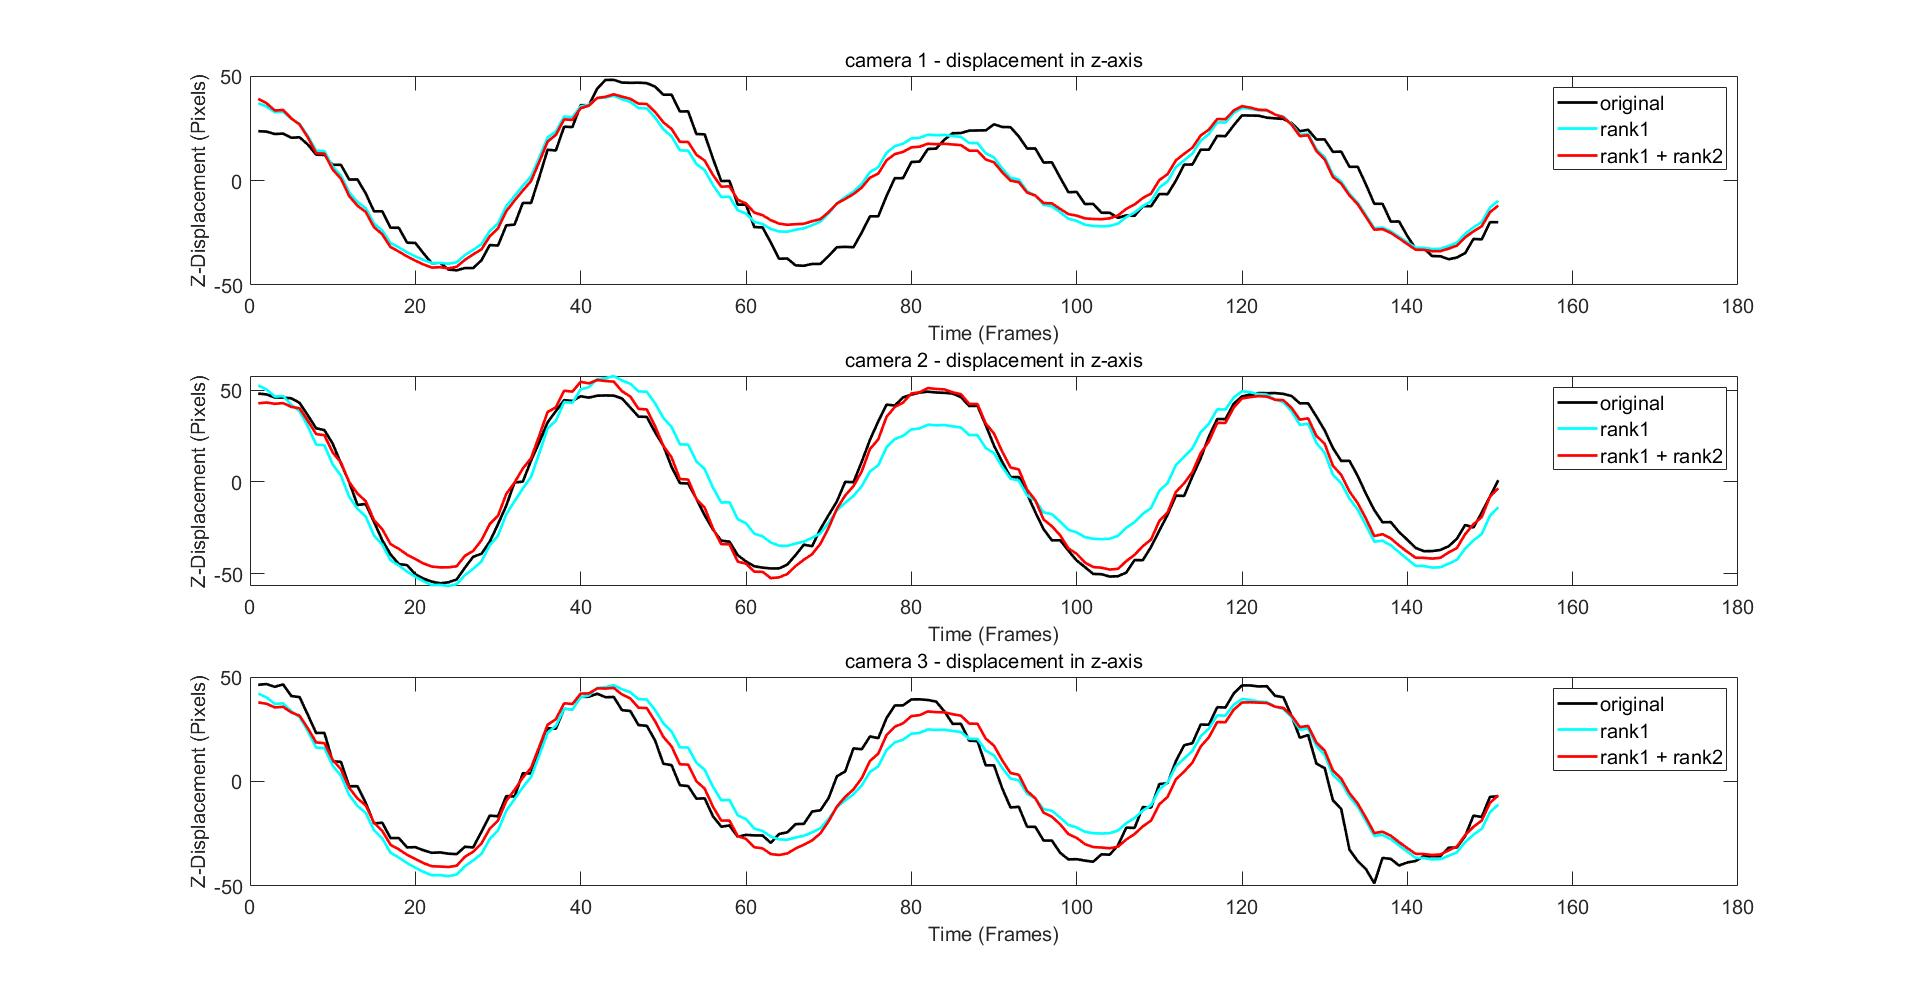
\includegraphics[width=8in]{case33.jpg}}
    \caption{Test 3: Horizontal Displacement - Comparison on the z-direction displacement between real and approximation}
\end{figure}
In this case, the original data produces sine wave curves in both the z-direction and the x-y plane. The interesting point is that, from Figure 9, the first component is about only ($63\%$), and the second component is about ($23\%$). However, we can see that the rank-1 approximation already provides a good approximation for the displacement in the Z-direction.

\subsection{Test 4: Horizontal Displacement and Rotation}
\begin{figure}[h]
    \centerline{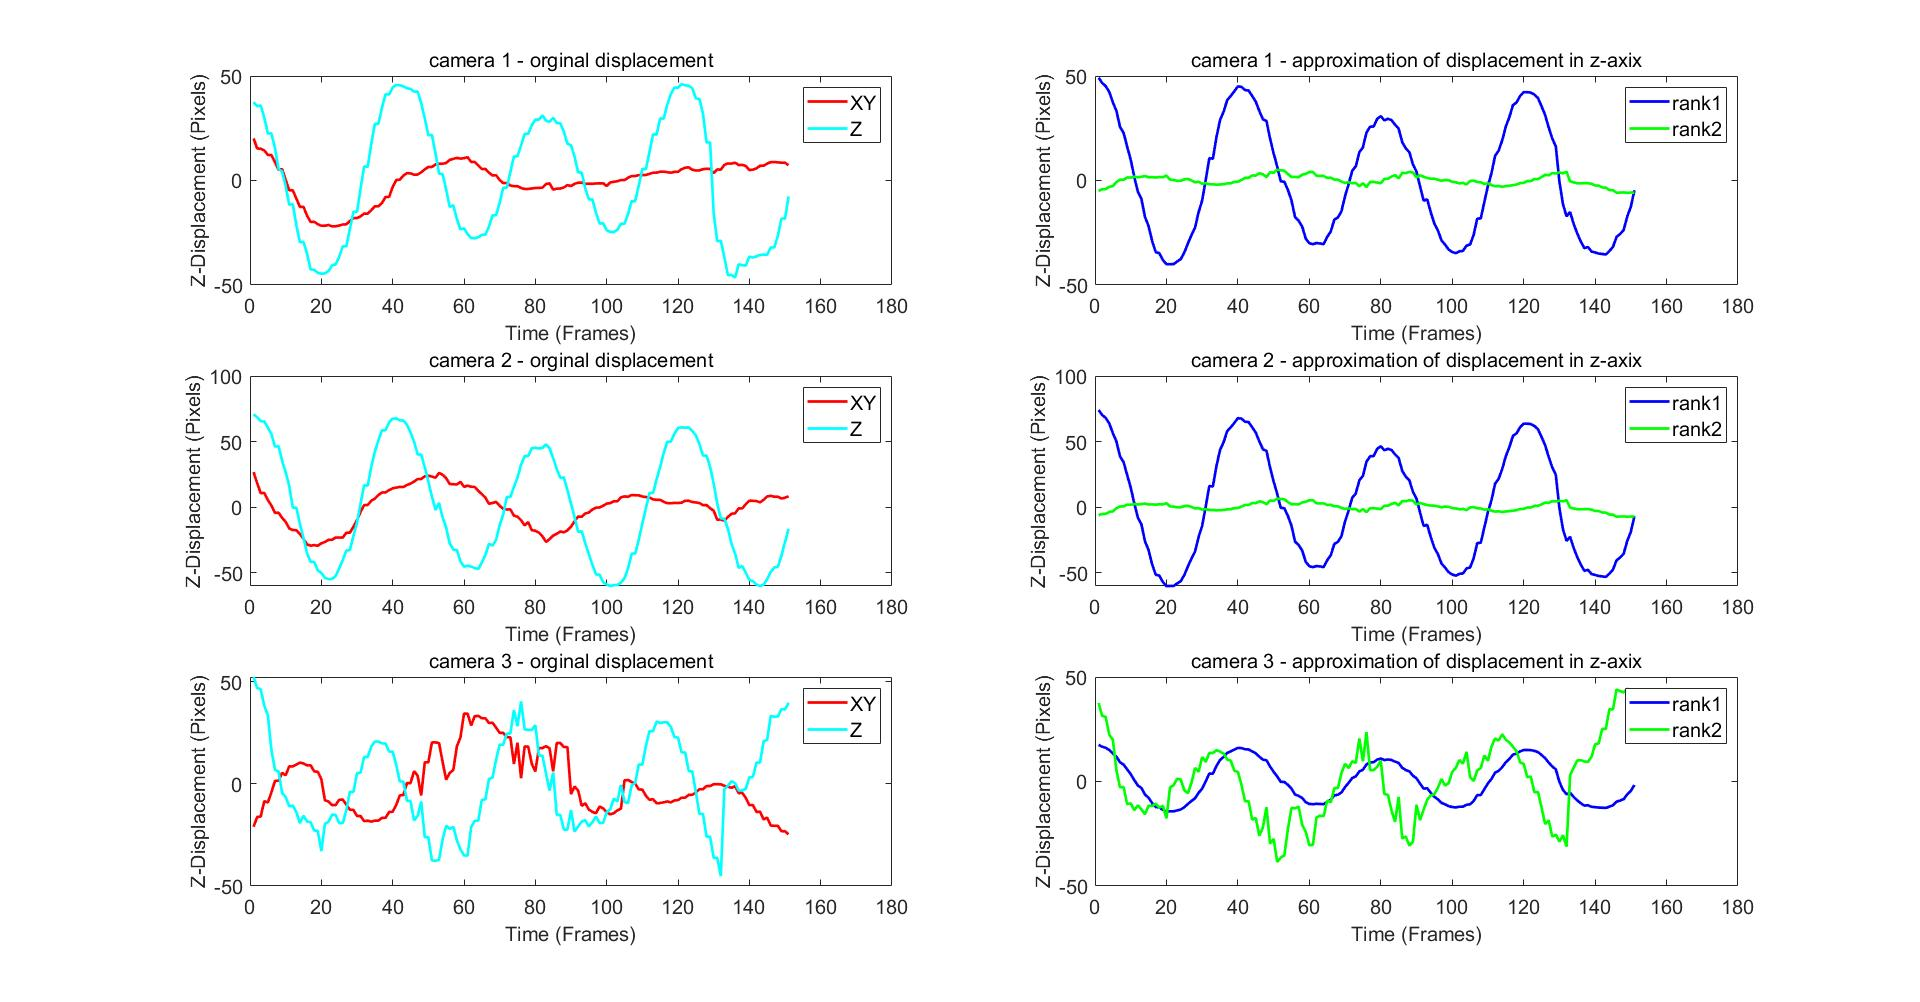
\includegraphics[width=8in]{case41.jpg}}
    \caption{Test 4: Horizontal Displacement and Rotation - The original displacement and its principle components}
    \centerline{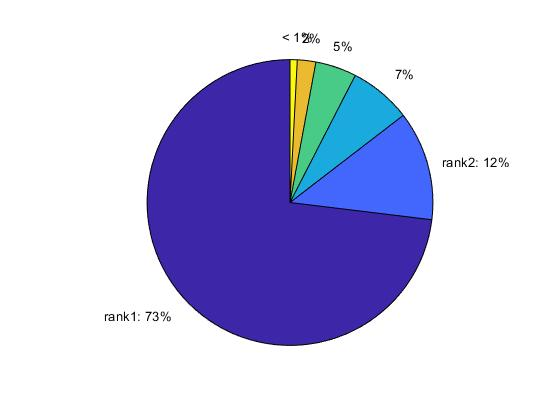
\includegraphics[width=3in]{case42.jpg}}
    \caption{Test 4: Horizontal Displacement and Rotation - The components of variance in the data}
\end{figure}
\begin{figure}[h]
    \centerline{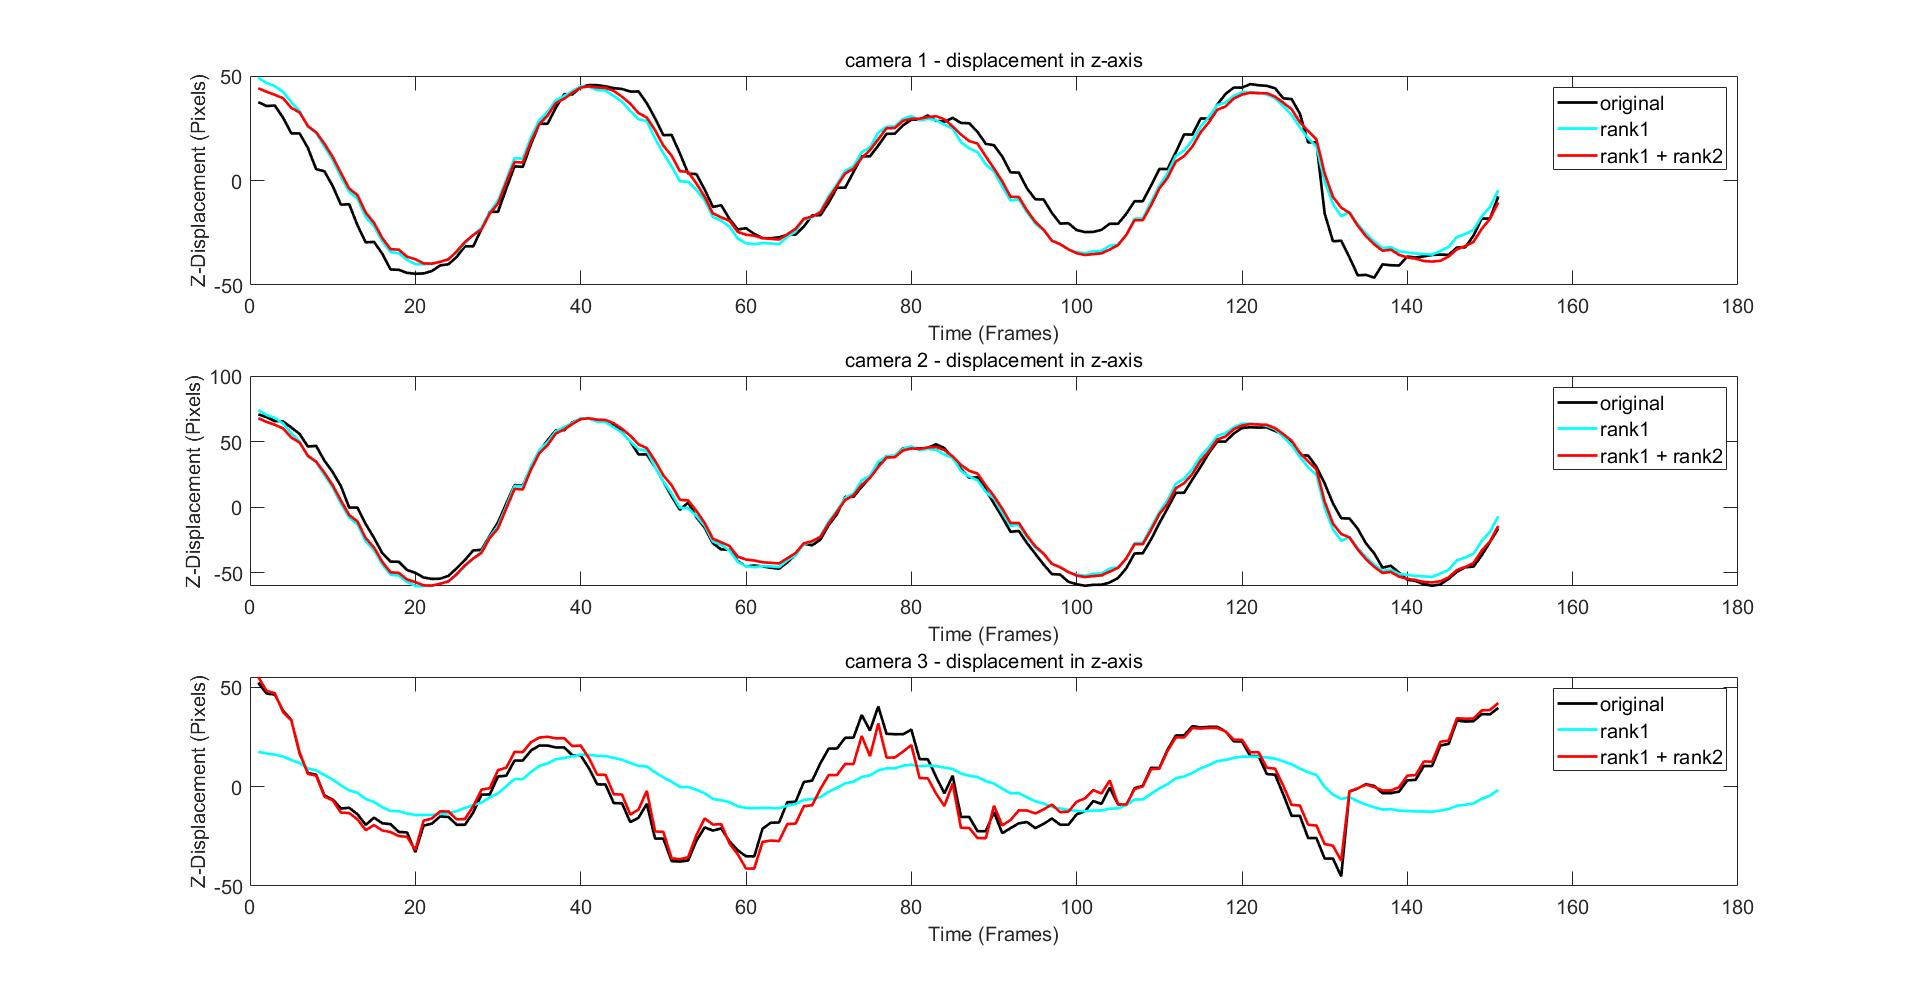
\includegraphics[width=8in]{case43.jpg}}
    \caption{Test 4: Horizontal Displacement and Rotation - Comparison on the z-direction displacement between real and approximation}
\end{figure}
In the last case, we can see a sine wave curve on the z-direction, but the displacement in the x-y plane is chaotic since the rotation was added to the system. Surprisingly, the rank-1 approximation takes up $73\%$ of the variance and is a good fit for the z-direction displacement.



\section{Summary and Conclusion}
The PCA is a powerful and practical tool to analysis data. In those study, we have shown that we are able to reproduces that data almost perfectly with the rank-1 and the rank-2 approximation. Beside, it also allows us to break down the data into difference components.

% Appendices
\begin{appendices}

% MATLAB Functions
\section{MATLAB Functions}
\begin{itemize}
    \item \texttt{[M, I] = max(img)} returns the linear indices of the 
    maximum values in matrix \texttt{img}
    \item \texttt{img = rbg2gray(img)} returns the image matrix in gray-scale.
\end{itemize}

% MATLAB Codes

\section{MATLAB Code}

\begin{verbatim}
%% clear all
clear all; close all; clc;

%% Setup
load('cam1_1.mat')
load('cam2_1.mat')
load('cam3_1.mat')

filter1 = zeros(480,640);
filter1(170:430, 300:420) = 1;

filter2 = zeros(480,640);
filter2(100:400, 235:400) = 1;

filter3 = zeros(480,640);
filter3(200:350, 250:450) = 1;

%% analyze the video
videos = {vidFrames1_1, vidFrames2_1, vidFrames3_1};
filters = {filter1, filter2, filter3};
thres = [250, 250, 247];
data = {[], [], []};

min_frame = 10000;
for i = 1:3
    min_frame = min(size(videos{i},4), min_frame);
end

for i = 1:3
    video = videos{i};
    filter = filters{i};
    
    
    for j = 1:min_frame
    	img = video(:,:,:,j);

        img = rgb2gray(img);
        img = double(img);
        
        img = img.*filters{i};
        
        indeces = find(img > thres(i));
        [Y, X] = ind2sub(size(img), indeces);
        
        data{i} = [data{i}; mean(X), mean(Y)];
    end
end
%%
data = [data{1}'; data{2}'; data{3}'];

% switch the order of rows,
data = [data(1:4,:);data(6,:);data(5,:)];

%% make sure they are in phase
new_data = [];
for i = 1:3
    X = data(2*i-1,:);
    Y = data(2*i,:);

    [M, I] = max(Y(1:50));
    new_data = [new_data; X(I:I+150); Y(I:I+150)];
    
end
test = data;
data = new_data;

%% premodify the data
X = [];
for i = 1:6
   X = [X; data(i, :) - mean(data(i, :))];
end

%% apply the SVD
n = length(X(1,:));
A = X / sqrt(n-1);

[U,S,V] = svd(A, 'econ');

X_rank1 = sqrt(n-1)*U(:,1)*S(1,1)*V(:,1)';
X_rank2 = sqrt(n-1)*S(2,2)*U(:,2)*V(:,2)';

S = diag(S).^2;

%% plot
clc; close all;

set(groot,'defaultLineLineWidth',2.0)


for i=1:3
    subplot(3,2,2*i-1)
    plot(1:n,X(2*i-1,:),'r-','MarkerSize',10); hold on;
    plot(1:n,X(2*i,:),'c-','MarkerSize',10); 
    title(sprintf('camera %d - orginal displacement', i))
    xlim([0 180]);
    legend('XY', 'Z')
    xlabel('Time (Frames)')
    ylabel('Z-Displacement (Pixels)')

    subplot(3,2,2*i)
    plot(1:n,X_rank1(2*i,:),'b-','MarkerSize',10);  hold on;
    plot(1:n,X_rank2(2*i,:),'g-','MarkerSize',10); 
    title(sprintf('camera %d - approximation of displacement in z-axix', i))
    xlim([0 180]);
    xlabel('Time (Frames)')
    ylabel('Z-Displacement (Pixels)')

    legend('rank1', 'rank2')
    
end
set(findall(gcf,'-property','FontSize'),'FontSize',15)


figure(2)
p = pie(S);
pText = findobj(p,'Type','text');
percentValues = get(pText,'String'); 
% labels = {'rank1: ';'rank2: ';'rank3: ';'rank4: ';'rank5: ';'rank6: '};
labels = {'rank1: ';'rank2: ';' ';' ';'  ';'  '};
combinedtxt = strcat(labels,percentValues); 
pText(1).String = combinedtxt(1);
pText(2).String = combinedtxt(2);
pText(3).String = combinedtxt(3);
pText(4).String = combinedtxt(4);
pText(5).String = combinedtxt(5);
pText(6).String = combinedtxt(6);

figure(3)
for i=1:3
    subplot(3,1,i)
    plot(1:n,X(2*i,:),'k-','MarkerSize',10); hold on;
    plot(1:n,X_rank1(2*i,:),'c-','MarkerSize',10); 
    plot(1:n,X_rank1(2*i,:) + X_rank2(2*i,:) ,'r-','MarkerSize',10);  

    title(sprintf('camera %d - displacement in z-axis', i))
    xlim([0 180]);
    legend('original', 'rank1', 'rank1 + rank2')
    xlabel('Time (Frames)')
    ylabel('Z-Displacement (Pixels)')

end

set(findall(gcf,'-property','FontSize'),'FontSize',15)


\end{verbatim}


\end{appendices}

\end{document}
